\documentclass[main.tex]{subfiles}
\begin{document}
\section{DARC Architecture}


The DARC is a virtual machine built with Solidity programming language \cite{soliditylangSolidityx2014}, and can be compiled and deployed to any EVM-compatible on local devnet, testnet or mainnet without contract code size limit(EIP-170). After the DARC protocol is successfully compiled and deployed to your blockchain, user can compose a program and send it to your DARC virtual machine using darc.js(the official Node.js SDK for deploying and interacting with your DARC) or ethers.js \cite{ethersDocumentation} with corresponding DARC Application Binary Interface(ABI). User can also read data and information from the deployed DARC in this way.

Figure \ref{fig:architecture} shows the overview of the DARC protocol. 

\begin{figure}
\centering
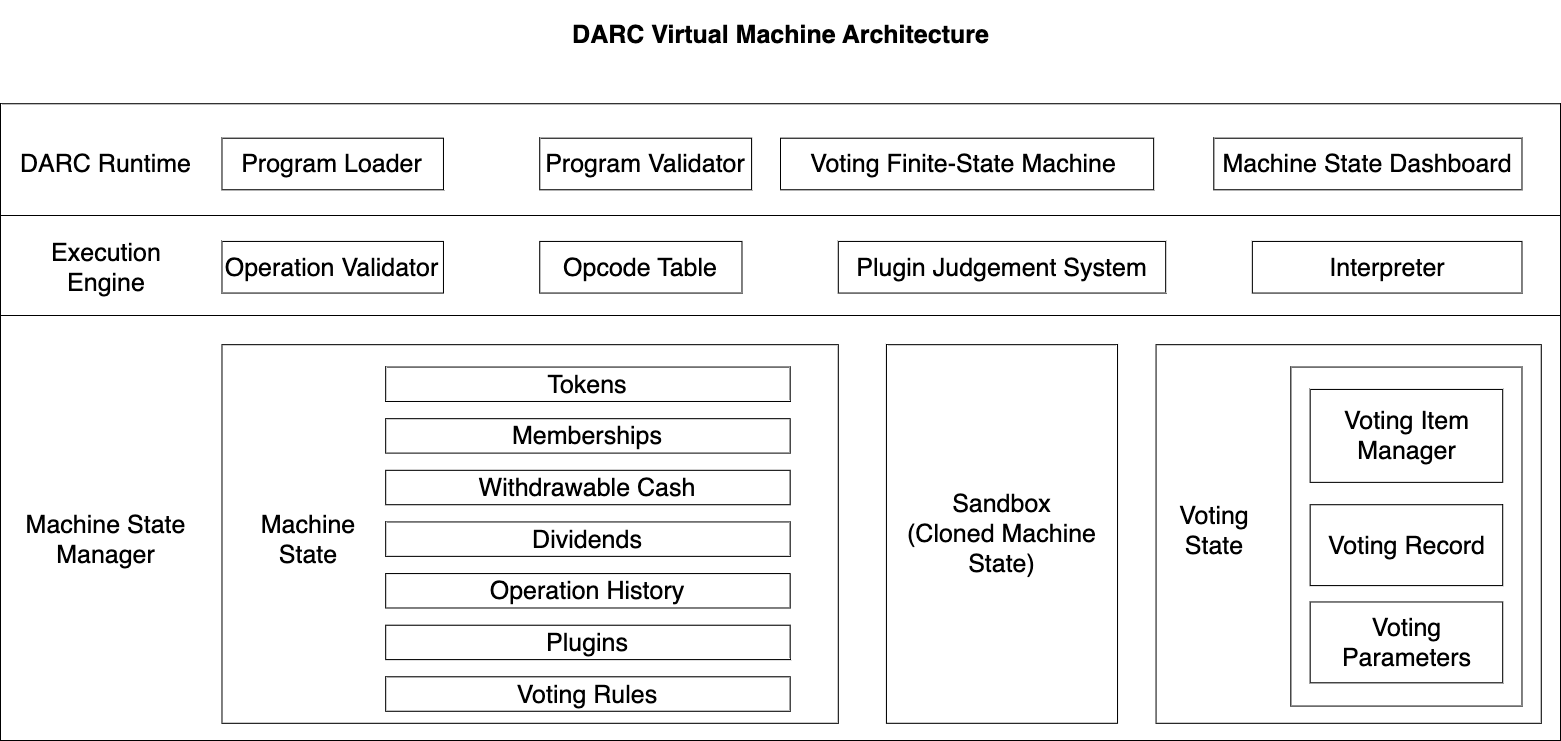
\includegraphics[width=1\linewidth]{architecture.png}
\caption{\label{fig:architecture}The architecture of DARC virtual machine.}
\end{figure}

\subsection{DARC Runtime}

The first level of DARC virtual machine is the Application Binary Interface (ABI) of the smart contract that allows user to compose and pass the programs into the DARC for executing. The program loader is the the entrace for all programs that are sent from user by using darc.js or ethers.js. 

\subsection{Program Loader}

Program loader is the module in the DARC runtime that receive the program from users. As the entrance of the DARC virtual machine, Program loader manages the whole process of handling the program, including validating the program, executing the program, determine the program compliance with the restriction plugin system, sending the program to the sandbox, starting a voting, ending a voting, pause a voting, refund unnecessary cash (the native tokens) back to the account balance. Program loader is the basic and fundamental module that handle the whole lifecycle of executing a program, as well as the state of the DARC for voting period.

\subsubsection{Program Validator}

Program validator is the module that checking if the program is valid, including calculate the total consumption of native tokens for each program, checking the basic syntax and parameters of each operation. When receiving the calculated consmuption of native tokens from program validator, the program loader will compare with the actual amount of native tokens user send with the program. If the value of native tokens sent is greater than the total comsumption, the program will be executed and the remaining amount of native tokens will be sent back to the user's balance; if the value of native tokens is less than the total comsumption, the program will be rejected directly, and all the native tokens will be refund into user's balance.

\subsubsection{Voting Finite-State Machine}

Voting Finite-State Machine is a Finite-State Macine(FSM) that handle the lifecycle of a voting procedure, including an idle state(all program can be submitted and executed), voting state(the process that only the program with operation ``vote'' can be executed), and a execution pending state(a period of time that allows user to execute a pending program that is approved by previous voting process). 

\subsubsection{Machine State Dashboard}

Machine State Dashboard is a set of interface that allows user to read all the necessary data and information from the DARC entity, including the basic information and parameters of DARC setup, the balances of multi-level token system for all token holders, the balance of withdrawable cash and dividends, the restriction plugins, the voting rules, and operation histories. All the functions in Machine State Dashboard are read-only and declared with ``view'' keyword, in which user can read the information without extra gas fee.

\subsection{Execution Engine}

The Execution Engine is the core module that check the validation via plugin system and execute each operation in both machine state and sandbox in the DARC virtual machine. It is similar like other intepreter for other Interpreted programming language, such like Java, Python, JavaScript, Perl, etc. 

After a program is validated and sent from runtime program loader, it will be directly passed into the execution engine. The Operation Validator is a module that checks if each operation is valid with right parameter syntax, such as the length of parameters and the types of parameters. After each opcode and corresponding parameters from the program is checked and validated by the operation validator, it will be ready to be checked by plugin judgement system and executed inside the opcode table and interpreter.

The opcode table is the module that analyze each opeartion with opcode and parameters and execute in the intepreter. When an operation is sent into the opcode table, it will be compared and sent to the interpreter with parameters and execute in the machine state or in the sandbox.

The plugin judgement system is the core module that check each operation and make the final judgement for the program, which decide the program should be accepted and executed in the machine state, rejected, executed in the sandbox and make the decision, pending and start voting for the final decision, or rejected after executed in the sandbox. The plugin judgement system reads two arrays of restriction plugins from the machine state: before-operation plugins array and after-operation plugins array. 

When the program passes the operation validator, it will be first checked by all the before-operation plugins: if all of the operations are approved by all before-operation plugins and allowed to be executed in the machine state, it will be passed to the opcode table and executed in the interpreter; if at least one of the operation is rejected by any before-operation plugin, the whole program will be rejected and the transaction will be reverted; otherwise, if none of the operations are rejected, but at least one of the operation is marked by any before-operation plugin as ``sandbox needed'', the legality of the program is not determined yet, and the whole program needs to be executed in the sandbox. 

After executed in the sandbox, the operation and the sandbox state will be checked by the after-operation plugins: if all of the operations and sandbox state are approved by all after-operation plugins, the program will be passed back to the opcode table and executed in the interpreter; if any of the operations or sandbox state is rejected by any after-operation plugin, the program will be rejected and the transaction will be reverted; otherwise, if none of the operations are rejected but at least one of the operation is marked by any after-operation plugin as ``vote needed'', then the program will be suspended and waiting for the final vote results, and will be allowed to executed after approved by the voting process and executed in the ``execution pending time''.

Since the sandbox also contains a copy of all before-operation plugins and after operation plugins, the after-operation sandbox check only uses the after-operation plugins in the current state. This is because the legality of a program should be only determined by the current machine state, including current plugin judgement system, and the machine state is allowed to be updated only by the program that is legal or approved by current machine state, current plugin judgement system and the voting result if necessary.

The workflow of the execution engine is shown in the figure \ref{fig:workflow}.

\begin{figure}
\centering
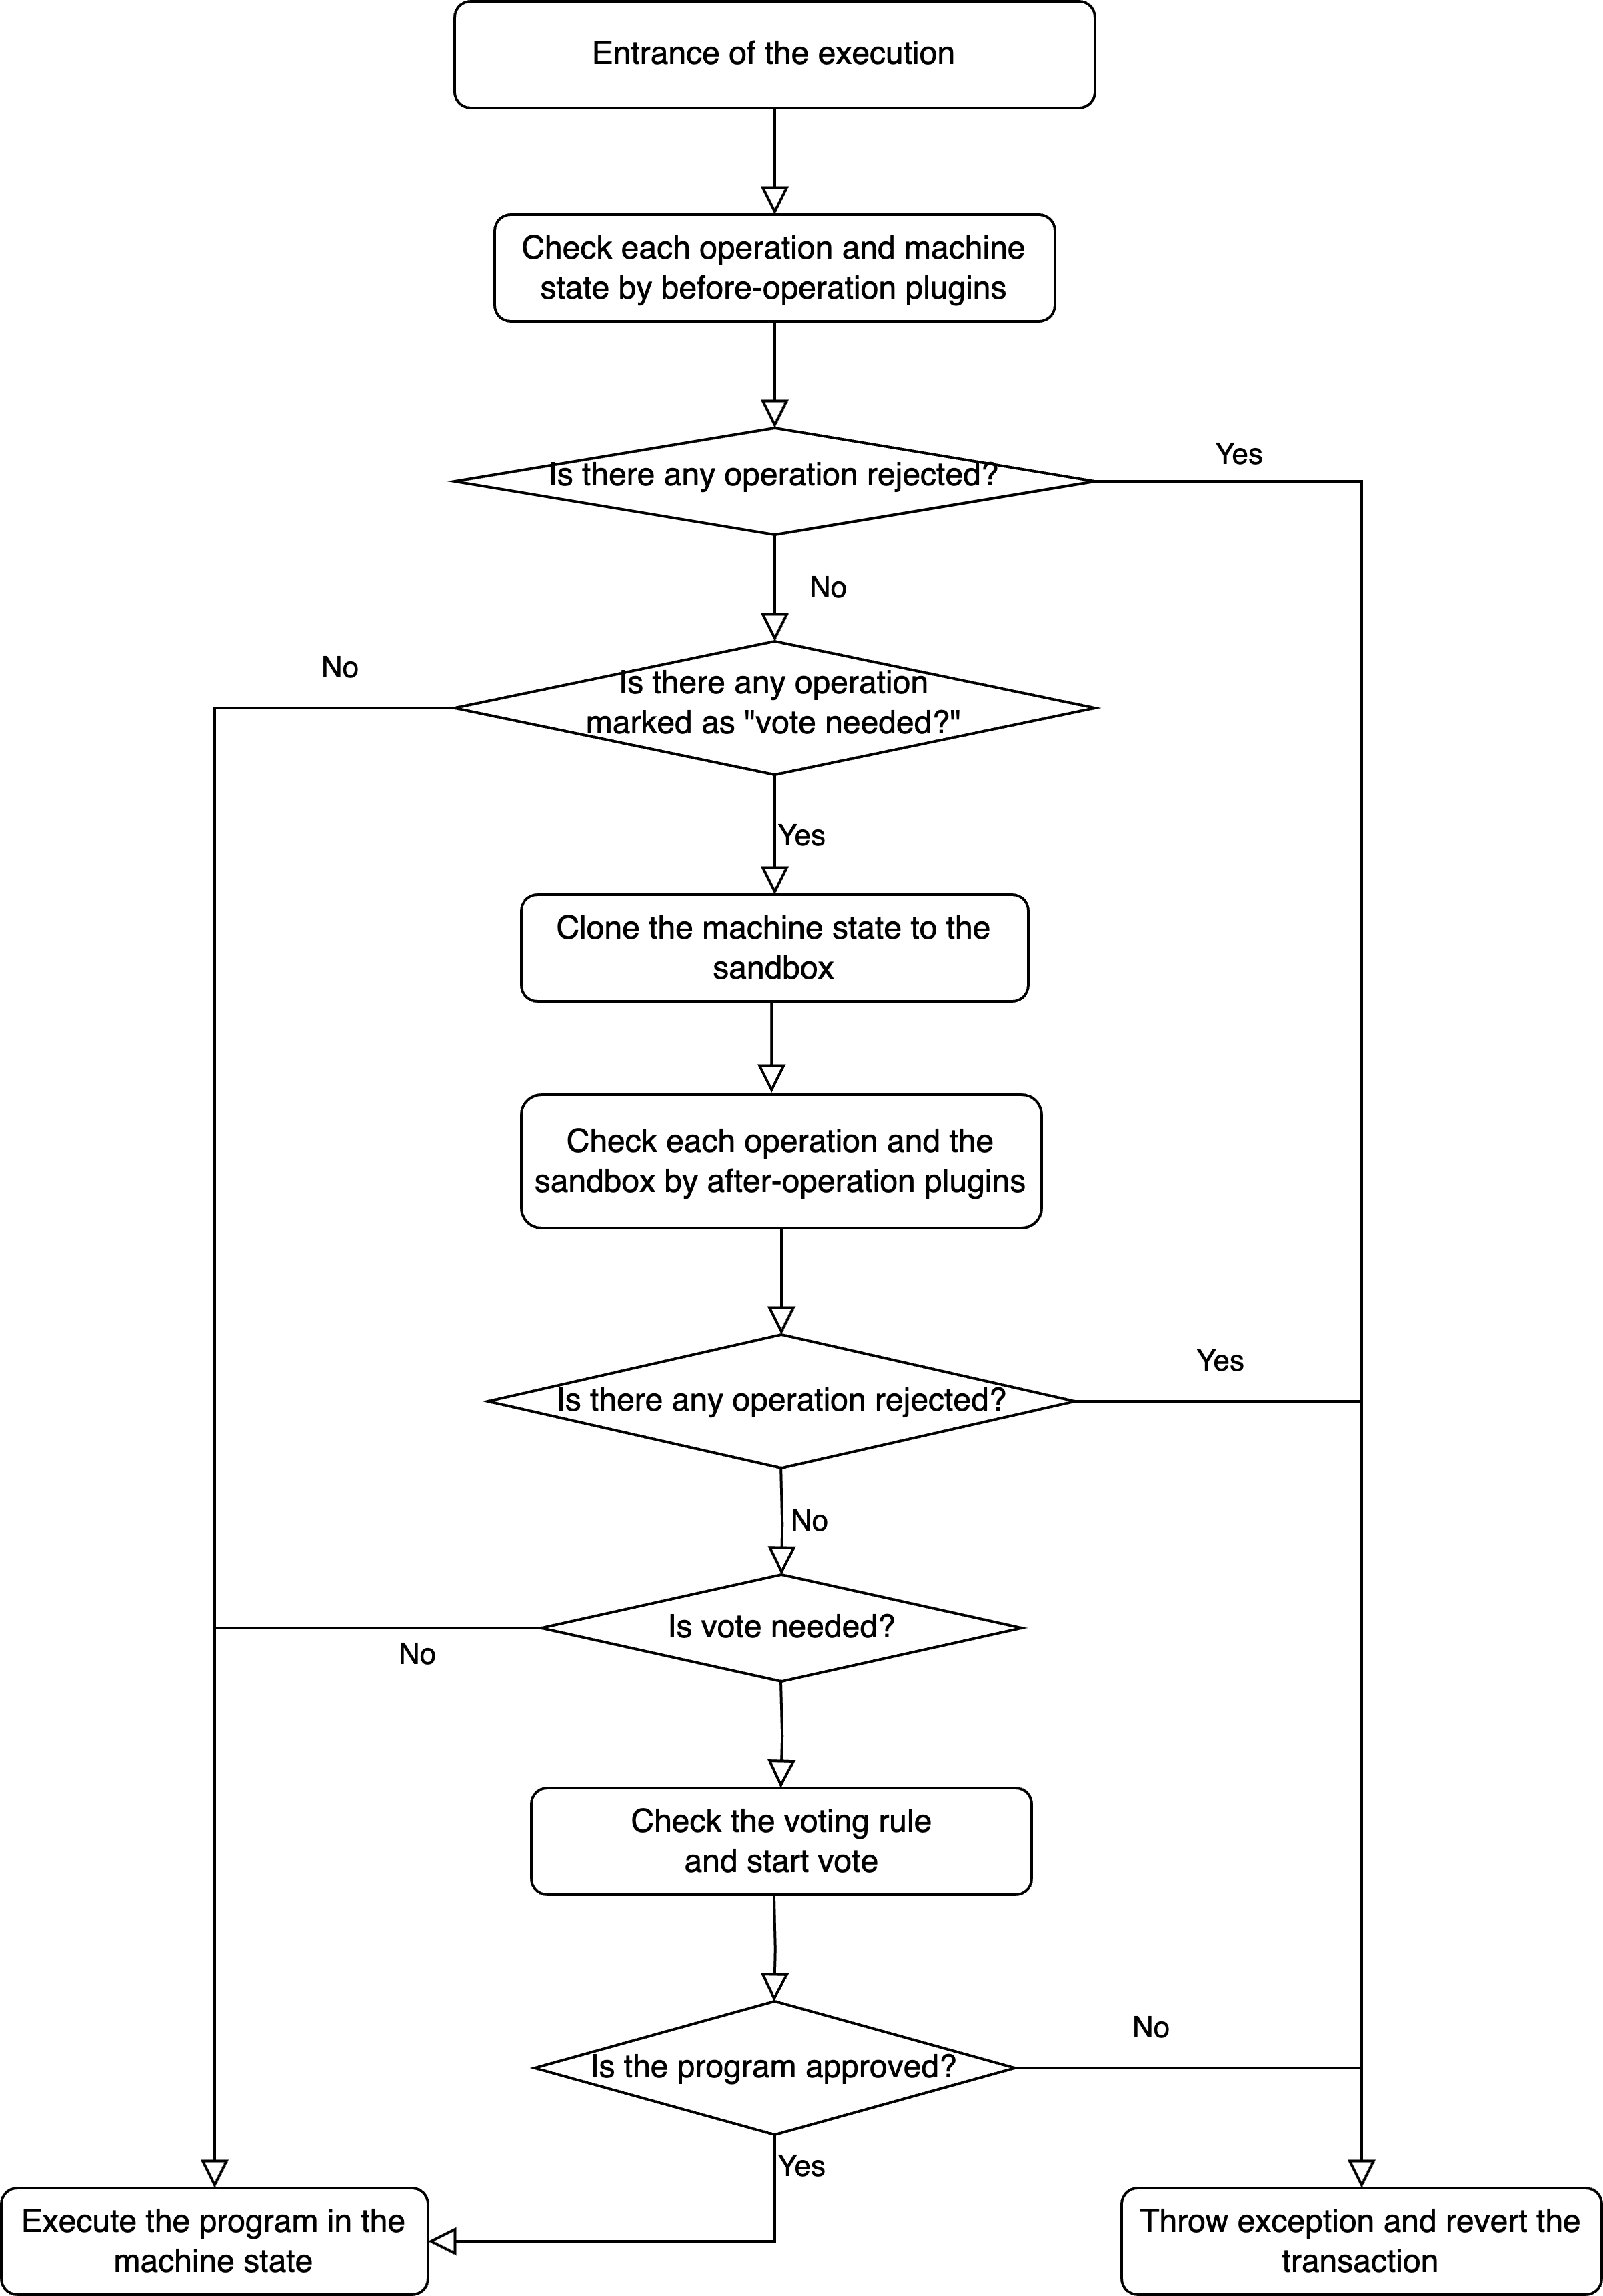
\includegraphics[width=1\linewidth]{execution_flow.drawio.png}
\caption{\label{fig:workflow}The workflow of execution engine.}
\end{figure}

\subsection{Machine State Manager}

Machine state manager is the module that store and manage all the state of the DARC. It contains three part: machine state, sandbox(the cloned machine state) and voting state. The machine state contains all the necessary state and assets of the DARC virtual machine, including token system, memberships, withdrawable cash and dividends balance, operation history, plugins and voting rules. 

\subsubsection{Tokens}

The token system is the most fundamental and core design in the DARC protocol. The machine state contains an array of tokens, each token contains different voting weight, dividend weight, token balance, token symbol(token information) and total supply.

The structure of each level token's information is stored in the machine state manager in following Solidity struct.

\begin{verbatim}
struct Token {
  uint256 tokenClassIndex;
  uint256 votingWeight;
  uint256 dividendWeight;
  mapping (address => uint256) tokenBalance;
  address[] ownerList;
  string tokenInfo;
  uint256 totalSupply;
  bool bIsInitialized;
}
\end{verbatim}

The token balance is a mapping from address to uint256. The key is the owner address of current level token, and the value is the number of tokens owned by this owner address. Also DARC maintains an array of address, ownerList, as the full list of all addresses with at least one token in current level of token.

\subsubsection{Memberships}

Membership is a a mapping from addresses to levels that enable the DARC to manage different address hierarchicially. The governance of DARC can make sure that different level of people can be assigned with different levels.

The reason that we introduce membership in DARC protocol is that users can develop different plugins to define different rules related to roles and addresses.

In the implementation of DARC Protocol, membership is defined as the following data structure:

\begin{verbatim}
/**
* The member list and internal role index number of each token owner,
* which can be used to represent the shareholders, co-founders, employees, 
* board members, special agents, etc.
*/
mapping (address => MemberInfo) memberInfoMap;

/**
 * The stock token owner information of the DARC protocol
 * This struct is used to store the role index number of each token owner
 */
struct MemberInfo {
  bool bIsInitialized;
  bool bIsSuspended;
  string name;
  uint256 role;
}
\end{verbatim}


\subsubsection{Withdrawable cash and dividends}

Withdrawable cash and dividends are two separate balance hashmaps. Operator can withdraw native tokens(like Ethereum) from both of the balance if the balance is not zero. For withdrawable cash, the only way to add withdrawable tokens to the address balance is to execute \texttt{BATCH\_ADD\_WITHDRAWABLE\_BALANCE} operation with target addresses and amounts of tokens. If the operation is approved, the corresponding amounts will be added to the balances. For dividends, the only way to add withdrawable tokens to the balance is to execute \texttt{OFFER\_DIVIDENDS} operation without any parameters. If the operation is approved, all token holders with dividendable tokens(tokens with dividend weight larger than 0) will receive the corresponding amount of dividends.

To withdraw the native tokens from the DARC to the address, the operator can execute \texttt{WITHDRAW\_CASH\_TO} to transfer withdrawable cash from balance to target addresses, or execute \texttt{WITHDRAW\_DIVIDENDS\_TO} to transfer dividends from balance to target addresses if the operations are approved.

\subsubsection{Operation History}

Operation history is a log system that contains each address with its all the corresponding operations, each operation with its latest timestamp. When a program is executed successfully, the timestamps of the operations contained in the program will be updated in the operation history. With the operation history, developers can set minimum time interval between each operations for a single address or for all members in the DARC.

Rule 1 is an example about using operation history to limit the operator to execute the same operation in a period of time:

\textbf{Rule 1}: We provide 10 ETH per month as the salary for both employee-level and manager-level address (level 4 \& 5 members).


For the Rule 1, we need to make sure that if the operator is assigned with a role level equals 4 or 5, the operation is adding withdrawable balance, the total amount of operation is less than or equal to 10 ETH(or 10000000000000000000 wei), and the operator did the same operation in more than 30 days(or 2592000 seconds), this operation will be approved and sandbox check can be skipped for this operation.

Here is an example plugin for Rule 1 designed in By-law Script:

\begin{verbatim}
const plugin_Rule_1 = 
{
    condition: (operation_name === BATCH_ADD_WITHDRAWABLE_BALANCE)
               & ( total_add_withdrawable_balance_up_to(10000000000000000000))
               & ( last_operation_by_operation_period_down_to(2592000)) 
               & ( (operator_membership_level_equals(4)) | (operator_membership_level_equals(5)) ) ,
    returnType: YES_AND_SKIP_SANDBOX,
    bIsBeforeOperation: true,
    level: 100,
    votingRuleIndex: 0,
    note: "Rule 1"
}
\end{verbatim}

Rule 1 does not restrict the target address of the \texttt{BATCH\_ADD\_WITHDRAWABLE\_BALANCE} operation. This is because operators are allowed to add 10 ETH to their own withdrawable cash, and they are also allowed to add to other addresses, as long as they do not exceed a total of 10 ETH of add withdrawable cash within 30 days.

\subsubsection{Plugins}

Plugins are the fundamental mechanism in DARC protocol, because all the rules and regulations need to be defined, transpiled and saved in DARC plugin system. There are two plugin arrays in the DARC protocol: before-operation plugins and after-operation plugins.


In the figure \ref{fig:workflow}, each program submitted to a DARC needs to be checked by all before-operation plugins, and if any operation of the program violates any before-operation plugin, the program will be rejected. 

If all operations are approved and no sandbox check needed, the DARC will execute the program directly; if one or some operations needs to be checked in the sandbox, the DARC will first copy all states from current DARC into the sandbox, then execute the whole program inside the sandbox, and double check the state of sandbox with after-operation plugins: if all the states and operations are approved by all after-operation plugins, the program will be approved and finally be executed in the real machine state; if one or some of the operations cannot be approved and need voting to make the further decision, the program will be suspended and the plugin system will start a voting process in the DARC, and the program will be approved and executed if and only if every pending operation is approved by the voting process, otherwise the program will be aborted and back to idle state.

Each plugin is composed with following items:
\begin{itemize}
\item Return type: the decision of the plugin when the condition is triggered, including \texttt{YES}, \texttt{VOTE\_NEEDED}, \texttt{NO}, \texttt{YES\_AND\_SKIP\_SANDBOX} and \texttt{SANDBOX\_NEEDED}.
\item Level: the priority of current plugin when the condition is triggered. When an operation triggers multiple plugins, the plugin system will make the final decision with the return type from the plugin with the highest level. Since each level only allows plugins with the same return type, this will make sure that each operation will get a certain judgement result from the plugin system.
\item Condition nodes: the \texttt{conditionNodes} is an array of condition nodes that represents the expression binary tree of this plugin. Each node can be a condition expression with parameters that validate a certain criteria, or a logical operators that combines two or multiple child nodes (condition expressions or logical operations) into a single condition expression. 
\item Voting rule index: the index number that pointing to a certain voting rule if the condition expression criteria is triggered and the return type of the plugin is \texttt{VOTE\_NEEDED}. If a voting process is needed, the judgement system will traverse all \texttt{VOTE\_NEEDED} plugins and create a voting process with multiple items with selected voting rules.
\item Note: the notes by plugin designers for future purpose.
\item Boolean flag \texttt{bIsEnabled}: the boolean flag that indicates if the plugin is enabled or not. Since the plugin is immutable in the whole life cycle, the operator cannot remove or modify the plugin after deployed successfully. The only way to disable a certain plugin is to set the boolean flag \texttt{bIsEnabled} from \texttt{True} to \texttt{False}. Also the plugin can be enabled by set it back to \texttt{True} if the operation is allowed.
\item Boolean flag \texttt{bIsInitialized}: the boolean flag that indicates if the plugin is successfully initialized. If \texttt{False}, the judgement system will skip this plugin.
\item Boolean flag \texttt{bIsBeforeOperation}: the boolean flat that indicates if the plugin is before-operation or after-operation plugin array. Although the before-operation plugins and after-operation plugins are stored and managed in two seperate arraies, this boolean will be double-checked when judgement system goes through each array. This field is required to make sure that each plugin object struct is aligned when constructing the plugin from By-law script and sending through the DARC program entrance.

\end{itemize}


The structure of a plugin is designed in Solidity with below struct:

\begin{verbatim}
struct Plugin {
  /**
   * the return type of the current condition node
   */
  EnumReturnType returnType;

  /**
   * the level of restriction, from 0 to the maximum value of uint256
   */
  uint256 level;

  /**
   * condition binary expression tree vector
   */
  ConditionNode[] conditionNodes;

  /**
   * the voting rule id of the current plugin if the return type is VOTE_NEEDED
   */
  uint256 votingRuleIndex;

  /**
   * the plugin note
   */
  string note;

  /**
   * the boolean that indicates whether the plugin is enabled or not
   */
  bool bIsEnabled;

  /**
   * the boolean that indicates whether the plugin is deleted or not
   */
  bool bIsInitialized;

  /**
   * the boolean that indicates whether the plugin is a before operation 
   * plugin or after operation plugin
   */
  bool bIsBeforeOperation;
  
}
\end{verbatim}

\subsubsection{Voting Rules Array}

Voting rules array is an array that stores all the voting rules for the DARC protocol. When a program is executed in the sandbox and being checked by the plugin judgement system, one or multiple operations may be pending and waiting for the voting results. During the voting process, all members are allowed to vote during the valid voting period. Each voting rule contains all the necessary requirements that starts the voting item.


\subsection{Sandbox}

The sandbox of DARC has exactly the same storage design as the machine state manager, including the token system, memberships, withdrawable cash, dividends, operation history, plugins and voting rules. For each program that cannot be approved by the before-operation plugins, the DARC machine state manager will first clone the machine state to the sandbox, execute the program in the sandbox, and make the decision based on the execution result and the sandbox state. 

\subsection{Voting State}

In the machine state manager, voting state is a standalone module that managing all voting-related properties. Voting item manager contains all the voting items in history, and each voting item contains the program waiting for the final voting result, the accumulated voting power and voting records for each address.

\end{document}